\chapter{Fluid Dynamics and Bernoulli's Equation}
This chapter is based on Munson Chapter 3.

\section{Definitions}
\paragraph{Streamline (SL)}
Streamlines are lines that are tangent to the velocity vector field at all points in space.

\begin{figure}[H]
	\centering
	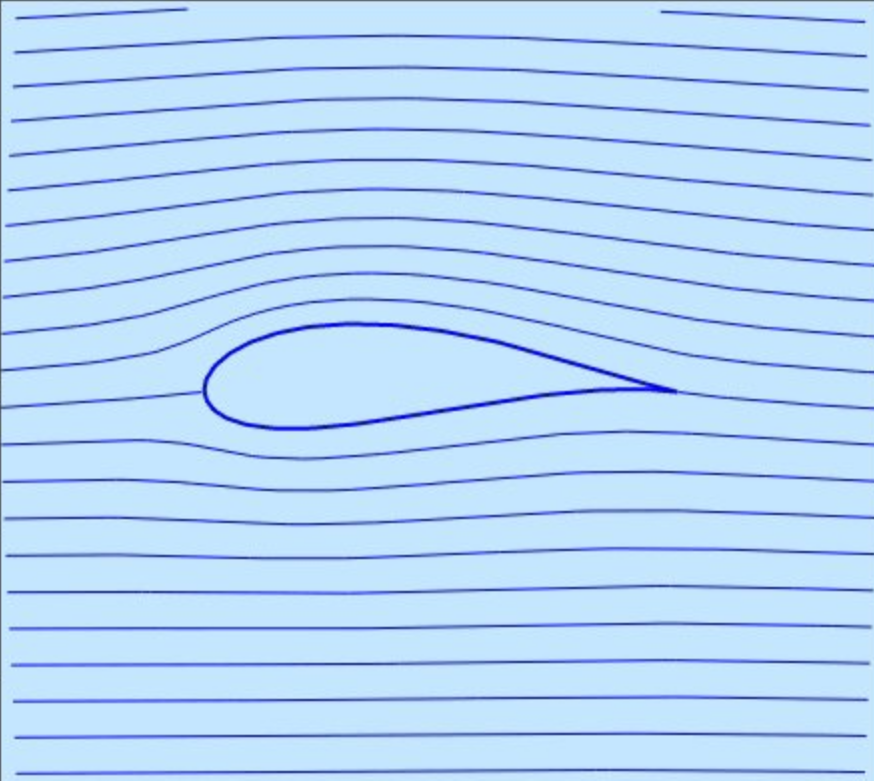
\includegraphics[width=0.3\linewidth]{Sketches/Airfoil}
	\caption{Streamlines along an airfoil}
	\label{fig:airfoil}
\end{figure}

\paragraph{Steady Flow}
When the velocity field $\vec v(\vec r, t)$ is time independent, we call the flow field \textbf{steady}. In this case the stream line is followed by fluid elements.


\section{Derivation of Bernoulli's Equation}

Recall newtons second law per unit volume \eqref{eq:newtons_second_law_per_unit_volume}:
\begin{equation*}
	-\nabla p - \rho g \hat k = \rho \vec a.
\end{equation*}

\begin{figure}[H]
	\centering
	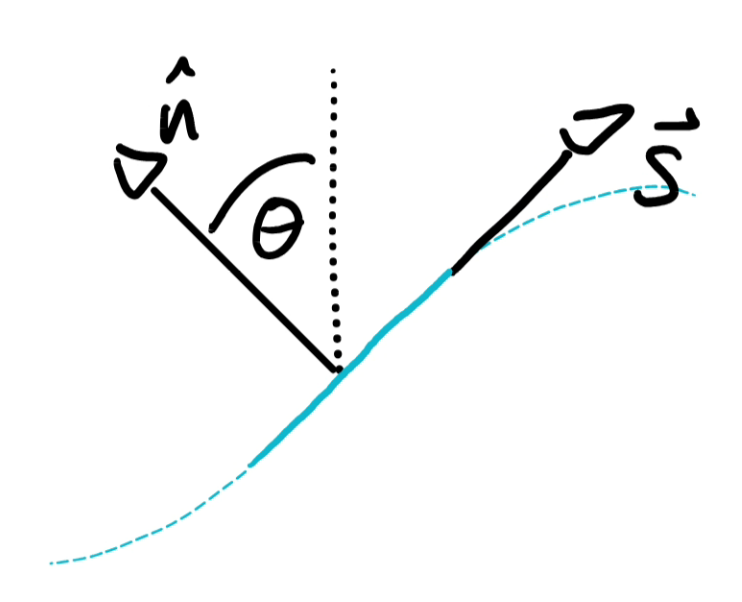
\includegraphics[width=0.3\linewidth]{Sketches/AlongStreamline}
	\caption{Coordinate system setup along a streamline.}
	\label{fig:alongstreamline}
\end{figure}

Along a stream line, (\ref{fig:alongstreamline}) with a normal with an angle $\theta$ to the vertical, we can use \eqref{eq:newtons_second_law_per_unit_volume} to state:


\begin{equation*}
	\begin{split}
		\vec a &= \frac{d\vec v}{dt} = a_s \hat s + a_n \hat n\\
		\text{in s-direction:}\quad a_s &= \frac{\partial v}{\partial s} \frac{\partial s}{\partial t} = \frac{\partial v}{\partial s} v\\
		\implies -\frac{\partial p}{\partial s} - \rho g\sin\theta &= \rho v\frac{\partial v}{\partial s}\\
		-\frac{\partial p}{\partial s} - \rho g \frac{\partial z}{\partial s} &= \rho \frac 12 \frac{\partial (v^2)}{\partial s}\\
		\frac 12 \rho \frac{\partial (v^2)}{\partial s} + \frac{\partial p}{\partial s} + \rho g \frac{\partial s}{\partial s} &= 0
	\end{split}
\end{equation*}

We integrate this along the streamline (in $s$), under the assumption that $\rho$ is constant:
\begin{equation}
	\boxed{\frac 12 \rho v^2 + p + \rho g z = C}
	\label{eq:bernoullis_equation}
\end{equation}
Which is \textbf{Bernoulli's Equation}, with units of energy per unit volume, or pressure. This equation is only valid if:
\begin{itemize}
	\item we have steady flow
	\item $\rho$ is constant
	\item we calculate along one streamline
	\item we can neglect viscosity / we have no shear forces.
\end{itemize}

Its first component ($v^2p/2$) is called \textbf{dynamic pressure}, the second ($p$) is the \textbf{static pressure}, the third ($\rho gz$) is called \textbf{head pressure} or \textbf{elevation pressure}. The first and second term combined is the \textbf{stagnation pressure}

\subsection{Stagnation Streamline}

\begin{figure}[H]
	\centering
	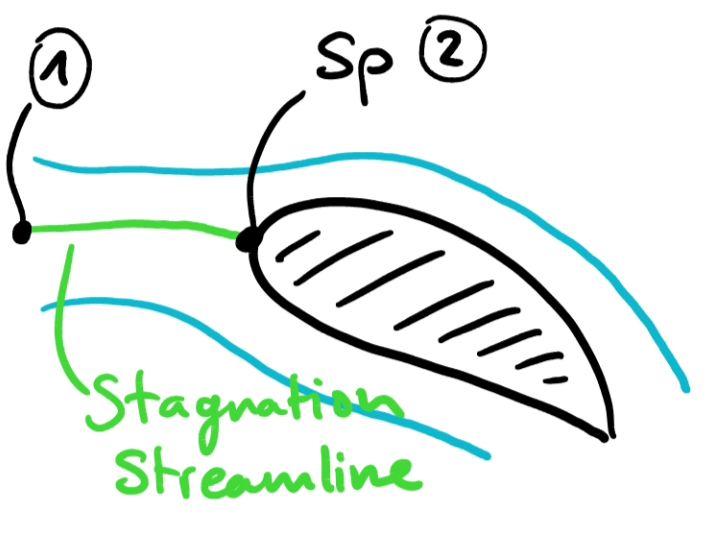
\includegraphics[width=0.3\linewidth]{Sketches/StagnationStreamline}
	\caption{The centred streamline that ends in the \textbf{Stagnation Point} (SP) is called \textbf{Stagnation Streamline}.}
	\label{fig:stagnationstreamline}
\end{figure}
Applying the Bernoulli's Equation for the stagnation streamline, yields:
\begin{equation*}
	p_1+\frac 12\rho v_1^2 = p_2 + \frac 12 \cancel{\rho v_2^2}^{\ast}
\end{equation*}
We ignored the $z$ term, because the pressure differences at flying altitude are negligible compared to the velocity of a plane. We cancel $\ast$ by the observation, that the velocity of the stream at the stagnation point is zero.

\subsection{Newton's 2nd law Across Streamlines}

Recall the coordinate system setup along a streamline (\ref{fig:alongstreamline}). To derive Bernoulli's Equation, we looked in the $s$-direction. If we look in the streamline-normal direction $\hat n$, we arrive at:
\begin{equation*}
	\begin{split}
		-\frac{\partial p}{n}-\rho g \cos \theta &= \rho \frac {v^2}R\qquad \left| \cos \theta= \frac{\partial z}{\partial n}\right.\\
		-\frac {dp}{dn}-\rho g \frac{dz}{dn} = \rho \frac{v^2}R\\
		-dp - \rho g \,dz &= \rho \frac{v^2}R dn
	\end{split}
\end{equation*}
Where $R$ is the \textbf{radius of curvature along $\hat n$}. We integrate the above term across the streamline, in $\hat n$ direction, yielding an important result:
\begin{equation}
		 \boxed{p + \rho gz + \rho \int \frac{v^2}{R}\,dn = C}
\end{equation}
Not knowing $R$ in the most cases makes this result unusable. However, if we have rectilinear (or nearly rectilinear) streamlines, the integration term disappears, as $R \to \infty$. From this we get the much more useable form:
\begin{equation}
	\boxed{p + \rho gz = C}
\end{equation}
\begin{figure}[H]
	\centering
	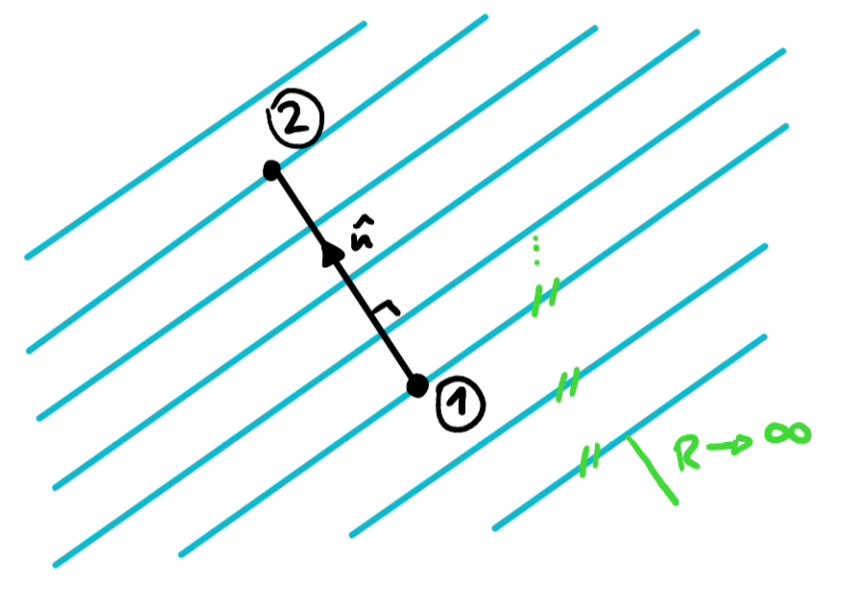
\includegraphics[width=0.4\linewidth]{Sketches/RectilinearStreamLines}
	\caption{All the streamlines are parallel to each other and straight ($R\to \infty$). We can take the difference between two points along the perpendicular direction $\hat n$.}
	\label{fig:rectilinearstreamlines}
\end{figure}
Applying this to a case like \ref{fig:rectilinearstreamlines} yields:
\begin{equation}
	p_2-p_1 = -\rho g (z_2-z_1) \implies p_1 = p_2+\rho gh
\end{equation}
Which can be recognized as one of the laws from hydrostatics.


\section{Applications}
\subsection{Pitot Tube}
To measure the speed with respect to the surrounding air, for example in a plane, pitot tubes are used. It consists of two tubes inside of each other. You can attach a gauge to measure the pressure difference between the two tubes, from which the speed can be found.
\begin{figure}[H]
	\centering
	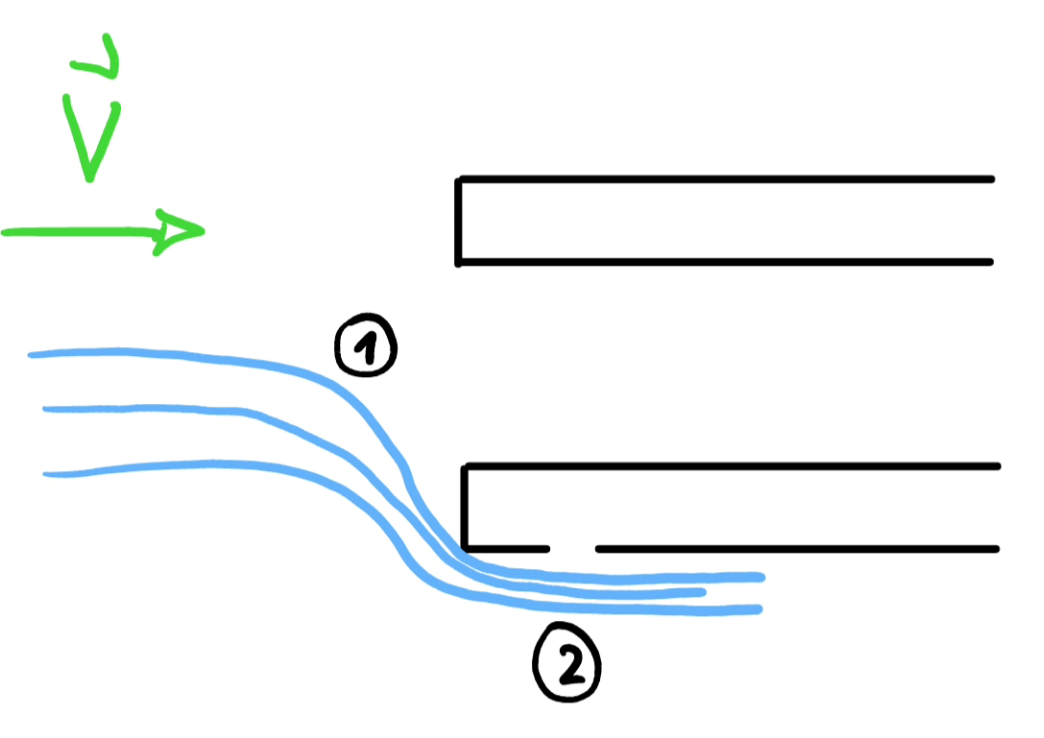
\includegraphics[width=0.4\linewidth]{Sketches/pitot_tube}
	\caption{A simplified representation of a pitot-tube.}
	\label{fig:pitottube}
\end{figure}

We can apply the Bernoulli equation \eqref{eq:bernoullis_equation} while neglecting gravity:
\begin{equation*}
	\frac 12\rho v^2+ p = C
\end{equation*}
Applying this to point 1 yields
\begin{equation*}
	p_1+\frac 12\rho v_1^2 = p+\frac 12 \rho v^2
\end{equation*}
We neglect the velocity difference (therefore $v_1=v$) in order to get the relation $p_1=p$. The measured pressure at point (1) is equal to the environment pressure.

For the second point we say that $v_2=0$ to get
\begin{equation*}
	p_2 = p + \frac 12 \rho v^2 
\end{equation*}

From the above relations we can summarize:
\begin{equation*}
	\begin{split}
		 p_2-p_1&=\frac 12 \rho v^2\\
		 v&=\sqrt{2\frac{p_2-p_1}\rho}
	\end{split}
\end{equation*}
We can conclude that by measuring the difference of pressure we can directly find the air speed.

\subsection{Venturi Tube}
\subsubsection{Mass Conservation and Steady Flow}
Consider a tube with walls that are defined by stream lines. 

\begin{figure}[H]
	\centering
	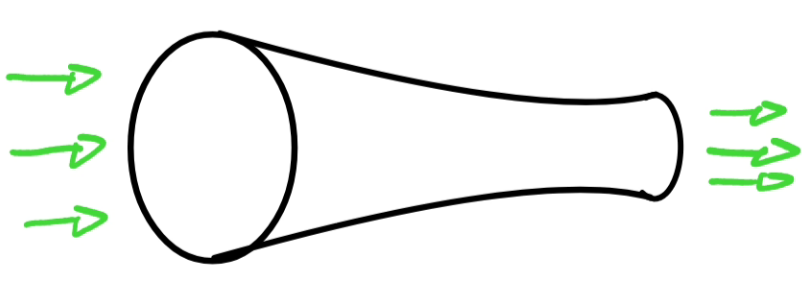
\includegraphics[width=0.4\linewidth]{Sketches/stream_tube}
	\caption{A stream tube: There are no walls, but we know that no mass is flowing through the borders, as they are defined through streamlines}
	\label{fig:streamtube}
\end{figure}

We can define the mass flow rate $\dot m$, where $[\dot m] = \frac{\mathrm{kg}}{\mathrm{s}}$.
and volume flow rate: $\dot V = v A$.
Using conservation of mass we write:
\begin{equation*}
	\rho_1 v_1 A_1 = \rho_2 v_2 A_2
\end{equation*}
for steady flow.

\subsubsection{Application of Mass Conservation}
\begin{figure}[H]
	\centering
	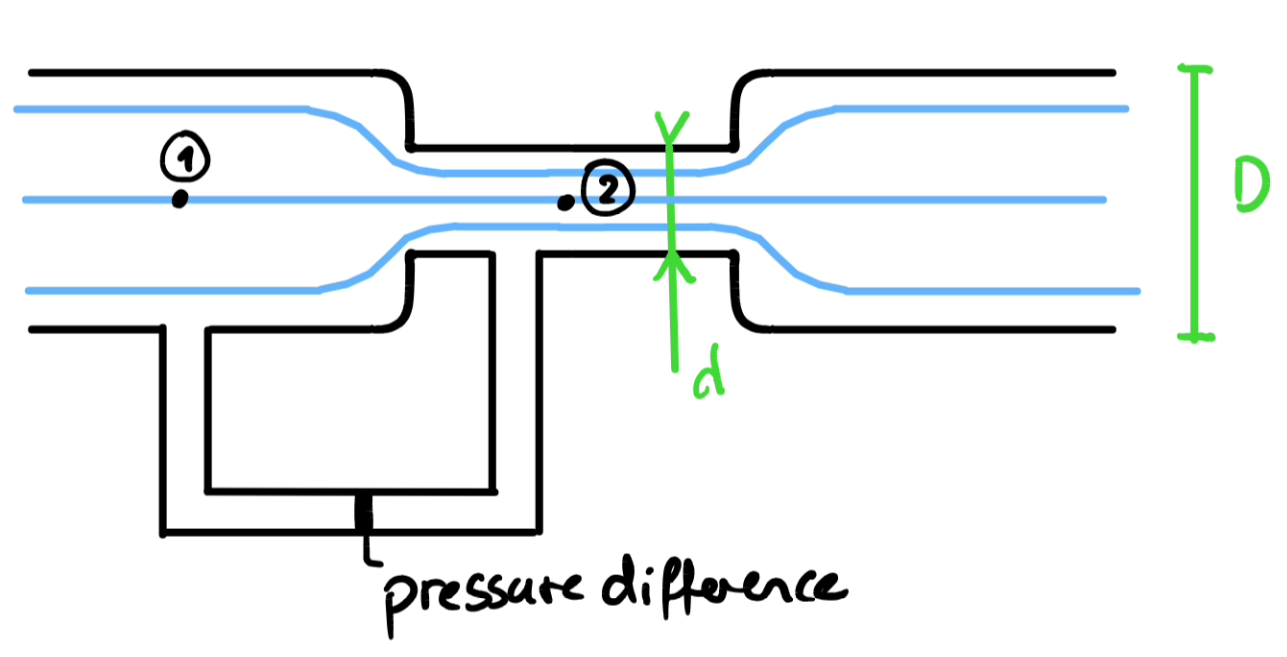
\includegraphics[width=0.7\linewidth]{Sketches/VenturiTube}
	\caption{}
	\label{fig:venturitube}
\end{figure}
We want to find the flow rate of a tube. For this, we add a thinner part and measure the pressure difference between (1) and (2). We apply the Bernoulli equation
\begin{equation*}
	 \frac 12 \rho v_1^2+p_1+\rho gz_1 = \frac 12 \rho v_2^2 + p_2 + \rho gz_2
\end{equation*}
to get the relationship
\begin{equation*}
	v_1^2+ 2 \frac {p_1-p_2}{\rho}=v_2^2
\end{equation*}
We need to apply mass or volume conservation in order to solve this any further, assuming  $\rho  = const$ we get that $v_1D^2 = v_2d^2$ which yields
\begin{equation*}
	v_2 = \sqrt{\frac{2(p_1-p_2)}\rho\div \left(\frac{D^4}{d^4}-1\right)}
\end{equation*}

\subsection{Free Jet}
Consider a bucket filled with a liquid. At the bottom we make a hole and allow the water to flow though.
\begin{figure}[H]
	\centering
	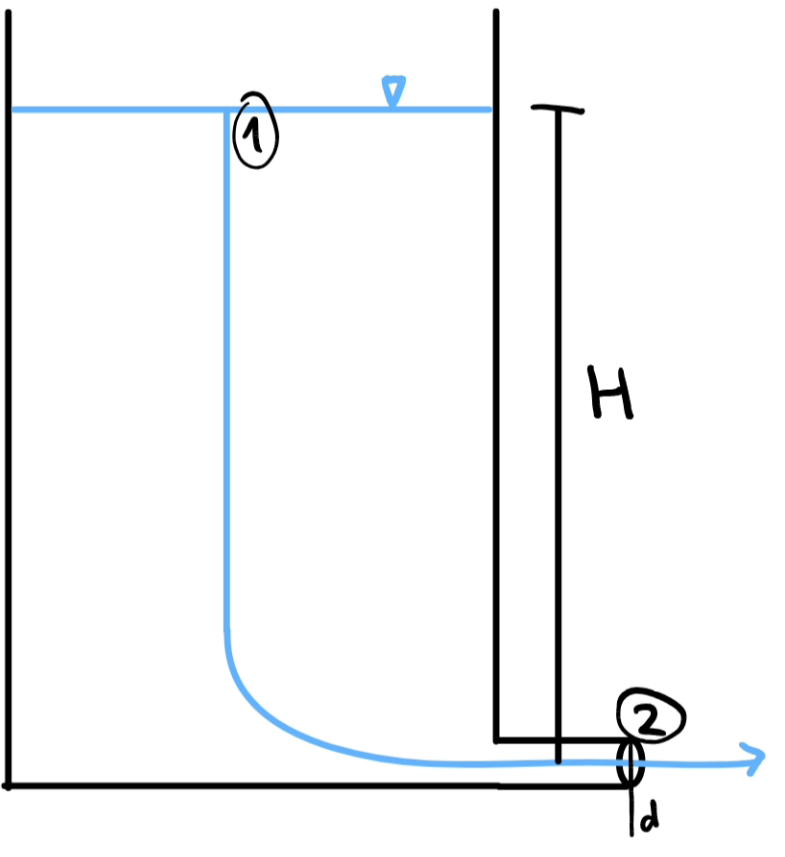
\includegraphics[width=0.3\linewidth]{Sketches/FreeJet}
	\label{fig:freejet}
\end{figure}

We choose a streamline from the centre to avoid shear forces that we would have if we were at the border. We assume that quasi-steady conditions apply (therefore fluid elements follow the same streamlines) for short time intervals or large buckets.

We apply Bernoulli's equation between (1) and (2) to get
\begin{equation*}
	\rho \frac{v_1^2}2+ \rho gz_1 + p_1 = \rho \frac{v_2^2}2+\rho gz_2 + p_2
\end{equation*}

we find that $z_1=H, z_2=0, v_1\approx 0, p_1=p_{atm}, p_2=p_{atm}$ simplifying 
\begin{equation*}
	\rho g H = \rho \frac{v_2^2}{2}\implies v_2^2=\sqrt{2gH}
\end{equation*}
Which is the same result as the speed of a free falling particle after height $H$.

To get the flow rate, we multiply the velocity by the cross-section:
\begin{equation*}
	\dot V = v_2\frac \pi 4 d^2=\frac{\sqrt{2gH}d^2\pi}4
\end{equation*}


\subsubsection{Vena Contracta}
Streamlines cannot abruptly change direction. Therefore the diameter of a stream after a contraption is always smaller or equal to the diameter of the hole:
\begin{figure}[H]
	\centering
	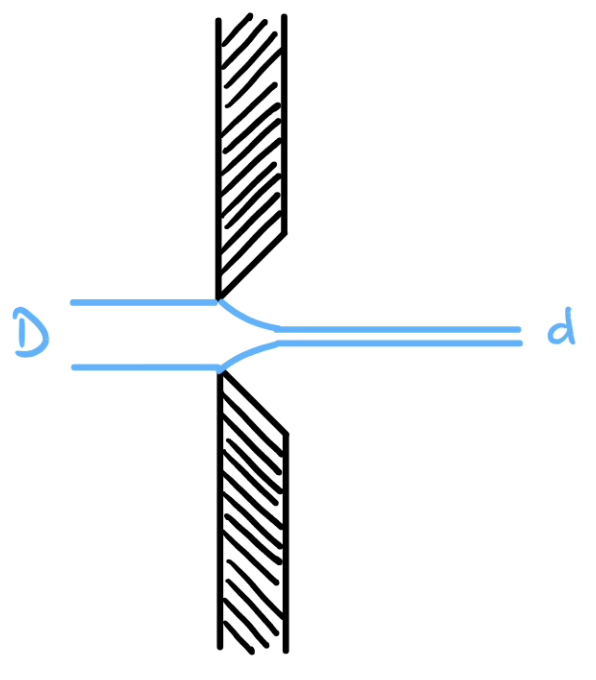
\includegraphics[width=0.3\linewidth]{Sketches/VenaContracta}
	\caption{}
	\label{fig:venacontracta}
\end{figure}
We define the contraction coefficient:
\begin{equation*}
	C_c = \frac{d^2}{D^2}\le 1
\end{equation*}
